\begin{pastexam}[label={px:ntu-112-dsa-07}]{臺大資工所 112 學年度 第 7 題}
（單選；5 分，答錯倒扣 1 分）

Given a list of binary trees $T=\{t_1,t_2,\ldots,t_7\}$ where each node is 0 or 1 shown as below,
we would like to insert these trees into a \textbf{linear-probing hash table} of length $N=11$. The
hash function $f(t)=g(h(t)) \bmod N$, where $h(t)$ is the binary sequence obtained from
\textit{in-order} traversal of tree $t$ and $g(\cdot)$ converts a binary sequence to a decimal
number. For instance, $g(\text{"1111111"})=127$. Here's the question: how many collisions occur
during the insertion process?

\begin{center}
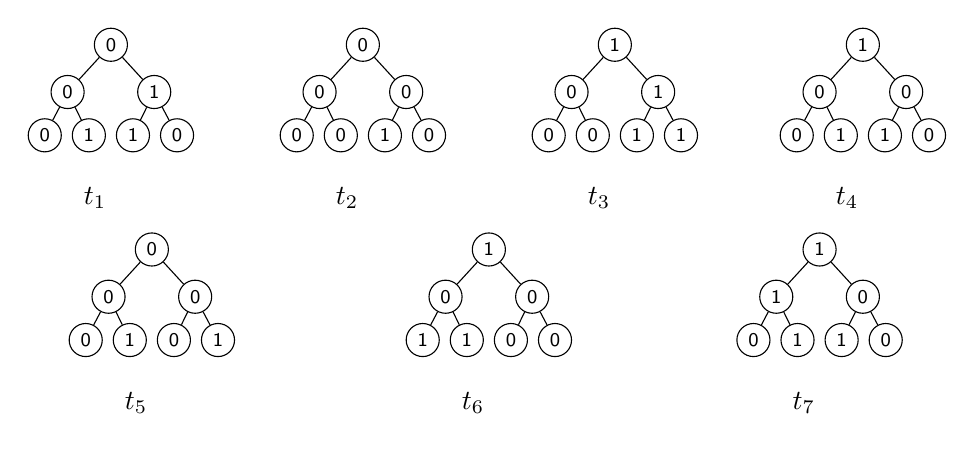
\begin{tikzpicture}[font=\sffamily\scriptsize,n/.style={circle,draw,inner sep=0pt,minimum size=4.2mm}]
\begin{scope}[shift={(0.00,0.00)}]
\node[n] (r) at (0,0) {0};
\node[n] (a) at (-0.55,-0.6) {0};
\node[n] (b) at (0.55,-0.6) {1};
\node[n] (l0) at (-0.84,-1.15) {0};
\node[n] (l1) at (-0.28,-1.15) {1};
\node[n] (l2) at (0.28,-1.15) {1};
\node[n] (l3) at (0.84,-1.15) {0};
\draw (r)--(a) (r)--(b) (a)--(l0) (a)--(l1) (b)--(l2) (b)--(l3);
\node[font=\normalsize] at (-0.2,-1.95) {$t_1$};
\end{scope}
\begin{scope}[shift={(3.20,0.00)}]
\node[n] (r) at (0,0) {0};
\node[n] (a) at (-0.55,-0.6) {0};
\node[n] (b) at (0.55,-0.6) {0};
\node[n] (l0) at (-0.84,-1.15) {0};
\node[n] (l1) at (-0.28,-1.15) {0};
\node[n] (l2) at (0.28,-1.15) {1};
\node[n] (l3) at (0.84,-1.15) {0};
\draw (r)--(a) (r)--(b) (a)--(l0) (a)--(l1) (b)--(l2) (b)--(l3);
\node[font=\normalsize] at (-0.2,-1.95) {$t_2$};
\end{scope}
\begin{scope}[shift={(6.40,0.00)}]
\node[n] (r) at (0,0) {1};
\node[n] (a) at (-0.55,-0.6) {0};
\node[n] (b) at (0.55,-0.6) {1};
\node[n] (l0) at (-0.84,-1.15) {0};
\node[n] (l1) at (-0.28,-1.15) {0};
\node[n] (l2) at (0.28,-1.15) {1};
\node[n] (l3) at (0.84,-1.15) {1};
\draw (r)--(a) (r)--(b) (a)--(l0) (a)--(l1) (b)--(l2) (b)--(l3);
\node[font=\normalsize] at (-0.2,-1.95) {$t_3$};
\end{scope}
\begin{scope}[shift={(9.55,0.00)}]
\node[n] (r) at (0,0) {1};
\node[n] (a) at (-0.55,-0.6) {0};
\node[n] (b) at (0.55,-0.6) {0};
\node[n] (l0) at (-0.84,-1.15) {0};
\node[n] (l1) at (-0.28,-1.15) {1};
\node[n] (l2) at (0.28,-1.15) {1};
\node[n] (l3) at (0.84,-1.15) {0};
\draw (r)--(a) (r)--(b) (a)--(l0) (a)--(l1) (b)--(l2) (b)--(l3);
\node[font=\normalsize] at (-0.2,-1.95) {$t_4$};
\end{scope}
\begin{scope}[shift={(0.52,-2.60)}]
\node[n] (r) at (0,0) {0};
\node[n] (a) at (-0.55,-0.6) {0};
\node[n] (b) at (0.55,-0.6) {0};
\node[n] (l0) at (-0.84,-1.15) {0};
\node[n] (l1) at (-0.28,-1.15) {1};
\node[n] (l2) at (0.28,-1.15) {0};
\node[n] (l3) at (0.84,-1.15) {1};
\draw (r)--(a) (r)--(b) (a)--(l0) (a)--(l1) (b)--(l2) (b)--(l3);
\node[font=\normalsize] at (-0.2,-1.95) {$t_5$};
\end{scope}
\begin{scope}[shift={(4.80,-2.60)}]
\node[n] (r) at (0,0) {1};
\node[n] (a) at (-0.55,-0.6) {0};
\node[n] (b) at (0.55,-0.6) {0};
\node[n] (l0) at (-0.84,-1.15) {1};
\node[n] (l1) at (-0.28,-1.15) {1};
\node[n] (l2) at (0.28,-1.15) {0};
\node[n] (l3) at (0.84,-1.15) {0};
\draw (r)--(a) (r)--(b) (a)--(l0) (a)--(l1) (b)--(l2) (b)--(l3);
\node[font=\normalsize] at (-0.2,-1.95) {$t_6$};
\end{scope}
\begin{scope}[shift={(9.00,-2.60)}]
\node[n] (r) at (0,0) {1};
\node[n] (a) at (-0.55,-0.6) {1};
\node[n] (b) at (0.55,-0.6) {0};
\node[n] (l0) at (-0.84,-1.15) {0};
\node[n] (l1) at (-0.28,-1.15) {1};
\node[n] (l2) at (0.28,-1.15) {1};
\node[n] (l3) at (0.84,-1.15) {0};
\draw (r)--(a) (r)--(b) (a)--(l0) (a)--(l1) (b)--(l2) (b)--(l3);
\node[font=\normalsize] at (-0.2,-1.95) {$t_7$};
\end{scope}
\end{tikzpicture}
\end{center}

(A)~0 \qquad (B)~1 \qquad (C)~2 \qquad (D)~3 \qquad (E)~4
\end{pastexam}

\begin{pastsoln}
答案是 (E)。

\textbf{第一步：中序序列和雜湊值。} 每棵樹都是 $7$ 個節點的完美二元樹。 把節點記成：根 $r$，左、右
子節點 $a, b$，四片葉子由左到右 $\ell_1, \ell_2, \ell_3, \ell_4$；中序走訪的順序是
$\ell_1, a, \ell_2, r, \ell_3, b, \ell_4$（資結書第~7.3~節）。 把讀到的位元當成二進位數，再對 $11$
取餘數：
\begin{center}
\small
\begin{tabular}{cccc}
\toprule
樹 & $h(t)$（中序） & $g(h(t))$ & $f(t) = g \bmod 11$ \\
\midrule
$t_1$ & \texttt{0010110} & $22$ & $0$ \\
$t_2$ & \texttt{0000100} & $4$ & $4$ \\
$t_3$ & \texttt{0001111} & $15$ & $4$ \\
$t_4$ & \texttt{0011100} & $28$ & $6$ \\
$t_5$ & \texttt{0010001} & $17$ & $6$ \\
$t_6$ & \texttt{1011000} & $88$ & $0$ \\
$t_7$ & \texttt{0111100} & $60$ & $5$ \\
\bottomrule
\end{tabular}
\end{center}
例如 $t_1$：$\ell_1 = 0$、$a = 0$、$\ell_2 = 1$、$r = 0$、$\ell_3 = 1$、$b = 1$、$\ell_4 = 0$，得
\texttt{0010110} $= 16 + 4 + 2 = 22$，$22 \bmod 11 = 0$。

\textbf{第二步：依序插入。} 線性探測：位置被占用就試下一格（資結書第~12.3~節）。
\begin{center}
\small
\begin{tabular}{cclc}
\toprule
插入 & 起始位置 & 探測過程 & 放在 \\
\midrule
$t_1$ & 0 & 0 空 & 0 \\
$t_2$ & 4 & 4 空 & 4 \\
$t_3$ & 4 & 4 被 $t_2$ 占（\textbf{碰撞}），5 空 & 5 \\
$t_4$ & 6 & 6 空 & 6 \\
$t_5$ & 6 & 6 被 $t_4$ 占（\textbf{碰撞}），7 空 & 7 \\
$t_6$ & 0 & 0 被 $t_1$ 占（\textbf{碰撞}），1 空 & 1 \\
$t_7$ & 5 & 5 被 $t_3$ 占（\textbf{碰撞}），6、7 也被占，8 空 & 8 \\
\bottomrule
\end{tabular}
\end{center}
最後的表：位置 $0$--$8$ 依序是 $t_1, t_6, -, -, t_2, t_3, t_4, t_5, t_7$，$9$、$10$ 空著。

碰撞指「要放的位置已經被占」。 以每次插入算，$t_3, t_5, t_6, t_7$ 四次插入發生碰撞，答案 $4$，
選 (E)。 注意 $t_7$ 的起始位置 $5$ 本來沒有別的樹雜湊到，是被 $t_3$ 探測過去占走的，這就是線性
探測的主要叢集。 如果把 $t_7$ 一路碰到的 $5, 6, 7$ 三格分開算，被占用的探測一共
$1 + 1 + 1 + 3 = 6$ 次，不在選項裡，所以題目的意思是「幾次插入發生碰撞」。
\end{pastsoln}
